%
% einleitung.tex -- Beispiel-File für die Einleitung
%
% (c) 2020 Prof Dr Andreas Müller, Hochschule Rapperswil
%
\section{Einleitung\label{pade:section:einleitung}}
\rhead{Einleitung}
Für praktische Berechnungen von Modellen in der Physik, Ingenieurwissenschaften und weiteren Feldern wird die Taylorreihe schon früh im Studium als ein nützliches Werkzeug gelehrt.
Leider liefert die Taylorreihe nicht immer die gewünschten Ergebnisse.
Dieses Paper beschäftigt sich mit der Padé-Approximation 
\begin{equation*}
[L/M]
=
\frac{P_{L}(x)}{Q_{M}(x)},
\end{equation*}
welche als ein weiteres Hilfsmittel zur Taylorreihe verwendet werden kann.
Die Padé-Approximation kann in manchen Fällen, in der die Taylorreihe keine genügenden Ergebnisse liefert, verwendet werden, um die Approximation deutlich zu verbessern.

 

\subsection{Das Taylorreihen Problem
\label{pade:Taylorfehler}}

Die klassische Antwort auf eine konvergierte Taylorreihe ist dass sie den Wert einer Funktion, welche beliebig oft abgeleitet werden kann, definiert. 
In der Praxis wird die Funktion jedoch nur mit immer längeren Polynomen approximiert.
Diese Methode kann bei praktischen Problemen auch einen sehr unerwünschten und limitierenden Effekt haben. 
Schauen wir das Beispiel 
\begin{equation*}
f(x)
=
\left(\frac{1+2x}{1+x}\right)^{\frac{1}{2}}
\approx
1+\frac{1}{2}x - \frac{5}{8}x^2+\frac{13}{16}x^3 -\frac{141}{128}x^4 +\frac{399}{256}x^5 - \frac{2353}{1024}x^6 + \frac{7205}{2048}x^7 \mp \cdots
\end{equation*}
an. 

Die originale Funktion $f(x)$ ist eine zwischen $0<x<\infty$ einfache und stetige Funktion, welche sich von $1$ zu $\sqrt{2}$ bewegt.
Die dazugehörige Taylorreihe ist jedoch nicht in der Lage bei einem Wert von $x>\frac{1}{2}$ zu konvergieren. 
Das Verhalten der originalen Funktion und dessen Taylorreihe ist in dem Graphen \ref{pade:prob1} ersichtlich. 

\begin{figure}
	\centering
	\subfigure[Plot von $f(x)$ und Taylorreihe 7. Ordnung.\label{pade:prob1}]{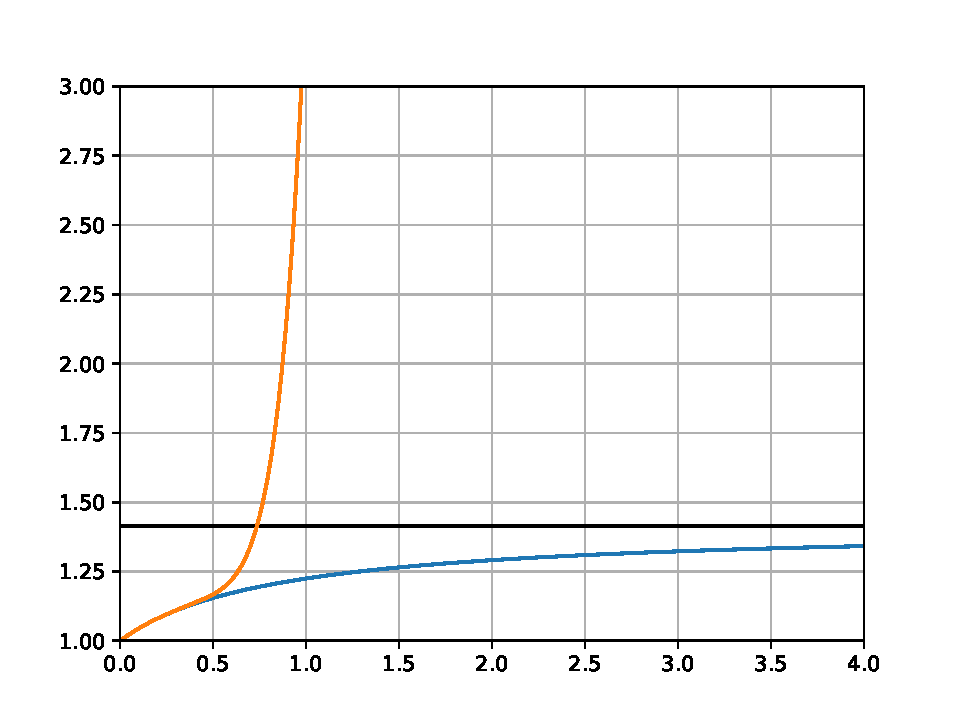
\includegraphics[width=0.45\linewidth]{./papers/pade/python/bilder/taylorProb1.pdf}}
	\subfigure[Fehler zwischen der Funktion und der Approximation.\label{pade:prob2}]{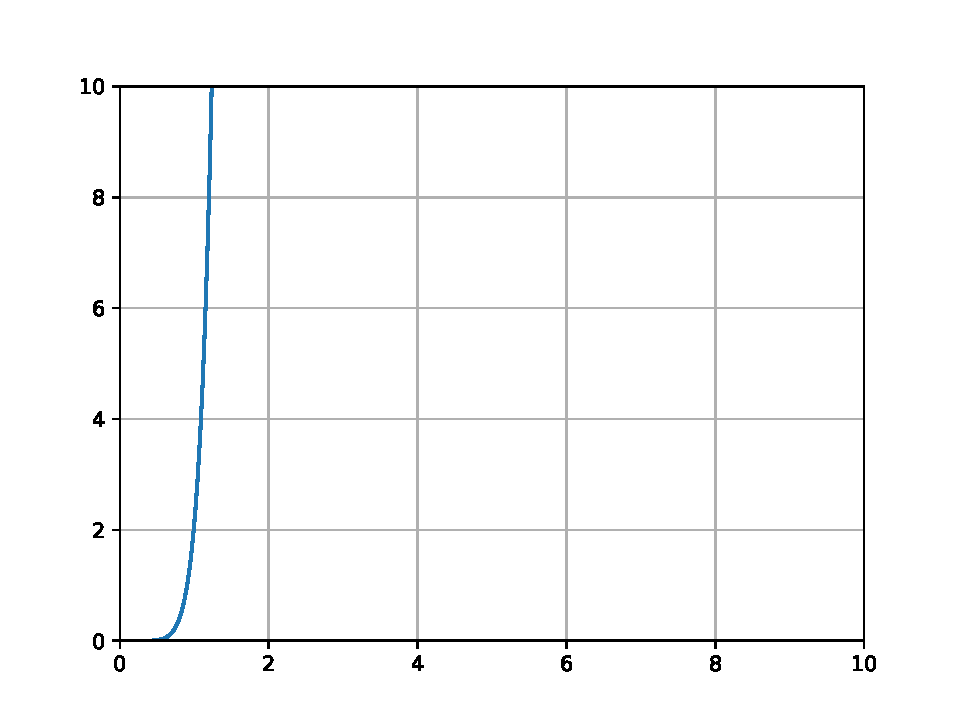
\includegraphics[width=0.45\linewidth]{./papers/pade/python/bilder/taylorProb3.pdf}}
	\subfigure[Plot von $f(x)$ und Padé-Approximation 3. Ordnung.\label{pade:prob3}]{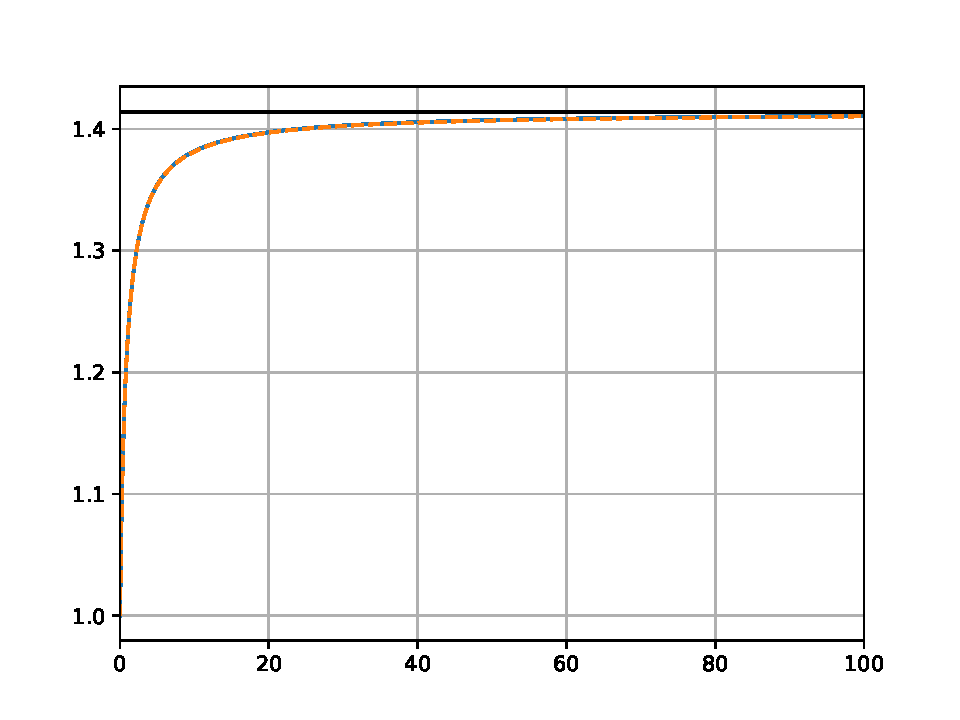
\includegraphics[width=0.45\linewidth]{./papers/pade/python/bilder/taylorProb2.pdf}}
	\subfigure[Fehler zwischen der Funktion und der  Padé-Approximation 3. Ordnung.\label{pade:prob4}]{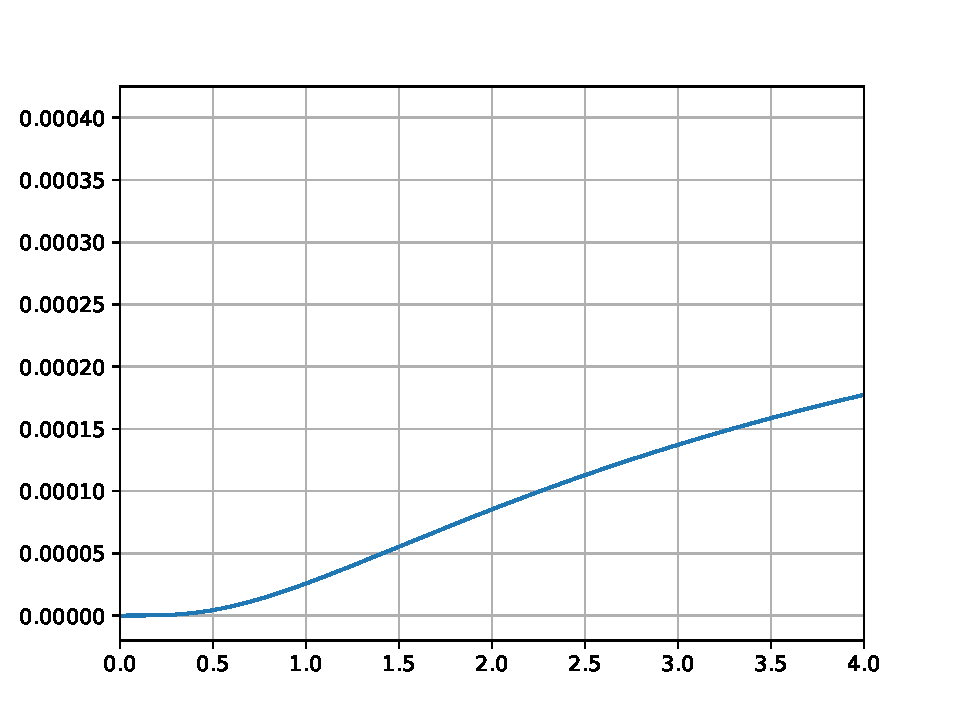
\includegraphics[width=0.45\linewidth]{./papers/pade/python/bilder/taylorProb4.pdf}}
	\caption{Visualisierung von der Funktion $f(x)$ und dessen Approximationen \label{pade:prob}}
\end{figure}
Die Padé-Approximation ist eine spezifische Art von rationalen Brüchen, welche eine Funktion approximiert.
Diese Art der Approximation führt oft zu einem besseren Resultat als eine Taylorreihe. 
Manchmal können mit der Padé-Approximation auch dann gute Ergebnisse gewonnen werden, wenn eine Taylorreihe wie in diesem Beispiel nicht konvergiert. 

Wenn man aus den Koeffizienten der Taylorreihe nun eine Padé-Approximation erstellt 
\begin{equation*}
\frac{P^{[3/3]}(x)}{Q^{[3/3]}(x)}
=
\frac{1+\frac{13}{4}x+\frac{41}{16}x^2}{1 + \frac{11}{4}x + \frac{29}{16}x^2} 
\end{equation*}
und diese Approximation bei immer grösser werdendem $x$ betrachtet
\begin{equation*}
\lim_{x \to \infty}
=
\frac{49}{29} = 1.413793103,
\end{equation*}
erhält man ein Ergebnis, welches sehr nahe an der original Funktion liegt. 
In der Grafik \ref{pade:prob3} ist gut ersichtlich wie viel besser sich die Padé-Approximation im Vergleich zu der Taylor-Approximation verhält.
Wenn die beiden Fehler der Taylorreihe \ref{pade:prob2} und der Padé-Approximation \ref{pade:prob4} zur originalen Funktion betrachtet werden, kann man sehen, dass die Padé-Approximation deutlich besser ist.
Dies obwohl von der originalen Funktion nicht mehr Informationen bekannt waren als bei der Taylorreihe, da das Polynom ja aus der Taylorreihe erstellt wurde.

In den folgenden Kapiteln wird nun aufgezeigt wie man eine Padé-Approximation erstellt inklusive einiger Beispiele.
Zum besseren Verständnis wird zuerst erklärt wie eine Potenzreihe einer Funktion herausgefunden werden kann.










